\documentclass[12pt,italian,a4paper,oneside,openright]{book}
\usepackage{url,amsfonts,epsfig}
\usepackage[italian]{babel}
\usepackage[utf8]{inputenc}
\usepackage{vmargin}
\usepackage{amsmath}
\usepackage{indentfirst}
\usepackage{graphicx}
\graphicspath{{img/}}
\usepackage[hyperindex]{hyperref} %per l'indice interattivo
\hypersetup{colorlinks=true, linkcolor=black} %per colorare i link
\DeclareGraphicsRule{.jpg}{jpg}{}{} %da commentare per il PDF
\setmarginsrb{35mm}{30mm}{30mm}{30mm}{0mm}{10mm}{0mm}{10mm}

%\documentclass{article}
\usepackage{listings}
\usepackage{xcolor}


% Impostazioni per lo stile del codice Java
% Impostazioni per il codice C
\lstset{
	language=C, % Linguaggio del codice
	basicstyle=\small\ttfamily, % Stile del testo base
	keywordstyle=\color{blue}, % Stile delle parole chiave
	commentstyle=\color{green!40!black}, % Stile dei commenti
	stringstyle=\color{orange}, % Stile delle stringhe
	numbers=left, % Posizione dei numeri di riga
	numberstyle=\tiny\color{gray}, % Stile dei numeri di riga
	stepnumber=1, % Incremento dei numeri di riga
	showstringspaces=false, % Mostra gli spazi nelle stringhe
	breaklines=true, % Spezza le linee lunghe
	frame=single, % Cornice intorno al codice
	framerule=0.5pt, % Spessore della cornice
	backgroundcolor=\color{gray!10}, % Colore dello sfondo
	captionpos=b, % Posizione della didascalia
	tabsize=3, % Dimensione del tab
	morekeywords={size_t, ssize_t}, % Parole chiave aggiuntive
}

\title{Relazione Reti}
\author{Lorenzo Di Palo}
\date{29/02/2024}

\begin{document}
	\pagenumbering{Roman}
	
	%%%% Opzione per interlinea 2
	\baselineskip 1.5em
	
	%% FRONTESPIZIO
	{ \thispagestyle{empty}
		
		\begin{center}
				
\includegraphics[scale=0.7]{img/logo.png}
		\end{center}
		\vskip 1cm \large \centerline{\textsc{Università degli Studi di
				Napoli ``Parthenope''}}
		
		\centerline {\textsc{Facoltà di Scienze e Tecnologie}}
		
		\centerline {\small\textsc{Corso di laurea in Informatica}}
		
	
		
		\vskip 0.5cm
		
		\large \centerline {\textsc{Documentazione Reti di Calcolatori}}
		
		\vskip 0.5cm
		
		\Large \centerline {Traccia:\\Università}
		
		
		\vskip 4.5cm
		
		
		\large
		\begin{minipage}[t]{7cm}
			\textsc{Docente}
			
			Emanuel Di Nardo\\
			
		\end{minipage}
		\hfill
		\begin{tabular}[t]{l}
			\textsc{Candidato} \\
			Di Palo Lorenzo\\
			Matricola: 0124002580
		\end{tabular}
		
		\vskip 2.0 cm \Large \centerline {Anno Accademico 2023-2024}
		\vfill \eject}
	
	
	\markboth{Indice}{Indice}
	\tableofcontents
	
	\newpage
	
	\pagenumbering{arabic}
	a


	\chapter{Descrizione dell'architettura} 
\newpage

\section{Architettura}
	Il sistema è costituito da 2 architetture client/server
	(I/O Multiplexing)
	\begin{itemize}
		\item \textbf{Server/Segreteria:} La prima connessione che avviene è questa.\\
		Quando viene eseguito lo script \texttt{start.sh}\\
		SERVER - SEGRETERIA - STUDENTE (\ref{studente}) vengono avviati\\
		il $Server$ attende che la $Segreteria$ si connetta.
		\item \textbf{Segreteria/Studente:} La seconda connessione avviene dopo che la prima non ha riportato errori.\\
		Se quest'ultima non riporta errori, \\
		$Segreteria$ attende l'inserimento delle Credenziali da parte dello $Studente$.
	\end{itemize}
	\newpage
\subsection{Componenti dell'architettura}
\begin{itemize}
	\item \textbf{Studente:}\label{studente} Fornisce interfaccia a linea di comando per:\\
	\begin{itemize}
	\item \textbf {Visualizza Appelli:}\\ Permette allo $Studente$ di scegliere tra la visualizzazione di tutti gli appelli nel suo corso o di un appello specifico.
	\item \textbf {Prenota Appello:}\\
	Richiede all'utente il nome del codice dell'esame al quale vuole prenotarsi e lo prenota nel primo appello disponibile.
	\item \textbf {Logout:}\\
	elimina le informazioni della sessione
	\end{itemize}
	
\end{itemize}

\begin{itemize}
	\item \textbf{Segreteria:}\label{segreteria}  Fornisce interfaccia a linea di comando per:
	\begin{itemize}
		\item \textbf{Gestire Studenti:}\\
		Gestisce le Richieste da parte di $Studente$
		\item \textbf{Inserire Appelli:}
		Inserisce nuovi appelli per esami esistenti in $Server$
	\end{itemize}
\end{itemize}

\begin{itemize}
\item \textbf{Server:}\label{server} Fornisce a $Segreteria$ la possibilità di:
	\begin{itemize}
		\item \textbf{Aggiunta Appello:}\\
		\item \textbf{Aggiunta Prenotazione:}\\
	\end{itemize}
\end{itemize}

\subsection{Flusso di Comunicazione}
 Server: Attende connessioni.\\
 Segreteria: Dopo aver stabilito una connessione con $Server$, $Segreteria$ è pronta a ricevere nuove connessioni.\\
 Studente: Dopo aver stabilito una connessione, $Studente$ invia le credenziali a $Segreteria$ per l'autenticazione. \\
 Una volta autenticato, $Studente$ può eseguire le Operazioni descritte in \ref{studente}.\\
 
 

	\chapter{Dettagli implementativi dei client/server} 
\newpage


\section{Studente}
\subsection{Connessione alla Segreteria}
$Studente$ stabilisce una connessione con $Segreteria$ utilizzando una socket, specificandone\\
Dominio($AF\_INET$)\\
Tipo ($SOCK\_STREAM$)\\
Protocollo (0)\\
\begin{lstlisting}[caption=Codice Connessione Socket, label=lst:ccs]
	
	if ((sockfd = socket(AF_INET, SOCK_STREAM, 0)) < 0) {
		perror("Errore nella creazione della socket!");
		exit(1);
	}
	servaddr.sin_family = AF_INET;
	if (inet_pton(AF_INET, argv[1], &servaddr.sin_addr) <= 0) {
		fprintf(stderr, "Errore inet_pton per %s\n", argv[1]);
		exit(1);
	}
	servaddr.sin_port = htons(PORT_CLIENT);
	
	if (connect(sockfd, (struct sockaddr *) &servaddr, sizeof(servaddr)) < 0) {
		perror("Errore nella connect: ");
		printf("\n");
		exit(1);
	}
\end{lstlisting}
\newpage
\subsection{Autenticazione}
$Studente$ inserisce credenziali e se non sono presenti nel database viene terminata l'esecuzione.
\begin{lstlisting}	[caption=Codice Autenticazione Segreteria, label=lst:cas]
	 printf("LOGIN\n");
	printf("Inserire matricola: ");
	scanf("%d", &mat);
	
	/**
	* Pulisco il buffer di input.
	*/
	while ((c = getchar()) != '\n' && c != EOF);
	
	printf("Inserire password: ");
	fgets(pass, sizeof(pass), stdin);
	pass[strlen(pass) - 1] = 0;
	
	write(sockfd, &mat, sizeof(mat));
	write(sockfd, pass, sizeof(pass));
	
	char state[255] = {0};
	read(sockfd, state, sizeof(state));
	
	printf("\nEsito login: %s", state);
	printf("\n");
	
	if (strcmp(state, "credenziali non corrette, accesso negato!") == 0) {
		exit(1);
	}
	
\end{lstlisting}
\newpage
\subsection{Scelta Operazione}
$Studente$ può effettuare una delle scelte riportate in \ref{studente}
\begin{lstlisting}[caption=Codice Scelta Operazione, label=lst:cso]
	printf("\nInserire il numero relativo all'operazione che si vuole effettuare:\n");
	printf("1 - Visualizza appelli disponibili\n");
	printf("2 - Prenota un appello\n");
	printf("3 - Logout\n");
	printf("Scelta: ");
	scanf("%d", &request);
	printf("\n");
	/*** pulisce buffer ***/
	write(sockfd, &request, sizeof(request));
	
\end{lstlisting}
\newpage
\subsection{Ottieni Risposta}
In base alla scelta effettuata, si ottiene una risposta dalla $Segreteria$. (Tentativo Formattazione Testo in C vano)
\begin{lstlisting}[caption=Codice Ottieni Risposta (Richiesta Appelli), label=lst:cor]
	read(sockfd, &num_rows, sizeof(num_rows));
	
	if (num_rows == 0) {
		printf("\nNon esistono appelli disponibili!\n");
	} else {
		printf("\nAppelli disponibili:\n\n");
		
		printf("| ID\tNome esame\tData | \n\n ");
		for (int i = 0; i < num_rows; i++) {
			read(sockfd, &id, sizeof(id));
			read(sockfd, name, sizeof(name));
			read(sockfd, date, sizeof(date));
			printf("%d\t%s\t%s\n", id, name, date);
			printf("-------------------------------\n");
		}
	}	
\end{lstlisting}



	\newpage
\section{Segreteria}
\subsection{Connessione al Server Universitario}
La connessione al server universitario rispecchia la connessione avvenuta in \ref{lst:ccs}

\subsection{Hosting}
La connessione da parte di $Studente$ richiede una socket che rimanga in ascolto in attesa di nuove connessioni\\
In questo caso la socket è "listenfd"\\
 \begin{lstlisting}[caption=Codice Ascolto Socket, label=lst:cass]
 	listenfd = getListenSocket(AF_INET, SOCK_STREAM, 0);
 	secaddr.sin_family = AF_INET;
 	secaddr.sin_addr.s_addr = htonl(INADDR_ANY);
 	secaddr.sin_port = htons(PORT_SERVER);
 	bindListener(listenfd, secaddr, sizeof(secaddr));
 	/**
 	* Mettiamo il server in ascolto, specificando quante connessioni possono essere in attesa venire accettate
 	* tramite il secondo argomento della chiamata.
 	*/
 	if ((listen(listenfd, 5)) < 0) {
 		perror("Errore nell'operazione di listen!");
 		exit(1);
 	}
 \end{lstlisting}
 \newpage
\subsection{Connessione al DB "UNIVERSITA"}
Se la connessione va a buon fine, $conn$ deterrà l'entry point per effettuare query sul DB\\
\begin{lstlisting}[caption=Codice Connessione DB, label=lst:ccdb]
	conn = mysql_init(NULL);
	if (conn == NULL) {
		fprintf(stderr, "mysql_init() fallita\n");
		exit(1);
	}
	if (mysql_real_connect(conn, "localhost", "nonnt66", "password", "universita", 3306, NULL, 0) == NULL) {
		fprintf(stderr, "mysql_real_connect() fallita: %s\n", mysql_error(conn));
		mysql_close(conn);
		exit(1);
	} else {
		printf("Connessione al database avvenuta con successo\n");
	}
\end{lstlisting}
\newpage


\subsection{Descrittori}
\begin{itemize}
\item Dichiarazione Descrittori:
\begin{itemize}
	Identifico 3 set di descrittori:
	\item \textbf{master\_set: } l'insieme di descrittori che verrà passato alla funzione select, settato inizialmente a zero.
	\item \textbf{read\_set: } l'insieme di descrittori che
	verifica quale descrittore è pronto in lettura
	\item \textbf{write\_set: } l'insieme di descrittori che
	verifica quale descrittore è pronto in scrittura\\
\end{itemize}
Inizialmente i vene impostato il massimo descrittore, scegliendo, tra la socket dello $Studente$ e la socket del $Server$
\begin{lstlisting}[caption=Codice Descrittori, label=lst:cd]
	fd_set read_set, write_set, master_set;
	int max_fd;
	FD_ZERO(&master_set);
	
	FD_SET(sockfd, &master_set);
	max_fd = sockfd;
	
	FD_SET(listenfd, &master_set);
	max_fd = max(max_fd, listenfd);
\end{lstlisting}
\newpage
\item Selezione Descrittori:
Si impostano i descrittori al valore della master\_set e si esegue la select per vedere se ci sono connessioni pronte
\begin{lstlisting}[caption=Codice Descrittori Select, label=lst:cds]
	if (select(max_fd + 1, &read_set, &write_set, NULL, NULL) < 0) {
		perror("Errore nell'operazione di select!");
	}
\end{lstlisting}
\item Verifica Descrittore Pronto:
Vado a verificare quale è il descrittore pronto in lettura/scrittura rispettivamente lato $Studente$, $Server$
 \begin{lstlisting}[caption=Codice Accettazione Studente - Lettura Scelta Studente, label=lst:caslss]
  if (FD_ISSET(listenfd, &read_set)) {
 	/**
 	* La system call accept permette di accettare una nuova connessione (lato server) in entrata da un client.
 	*/
 	if ((client_sockets[dim].connfd = accept(listenfd, (struct sockaddr *) NULL, NULL)) < 0) {
 		perror("Errore nell'operazione di accept!");
 	} else {
 		/**
 		* Si aggiunge il descrittore legato alla nuova connessione da uno studente all'interno dell'array di
 		* descrittori master_set e si ricalcola il numero di posizioni da controllare nella select.
 		*/
 		FD_SET(client_sockets[dim].connfd, &master_set);
 		max_fd = max(max_fd, client_sockets[dim].connfd);
 		/*** esegue oprazioni SQL ***/
 		/*** Itera sui client connessi ***/
 		if (FD_ISSET(client_sockets[i].connfd, &read_set) && client_sockets[i].connfd != -1) {
 			read(client_sockets[i].connfd, &behaviour, sizeof(behaviour));
 \end{lstlisting}
 
\end{itemize}





	\newpage
\section{Server}
\subsection{Operazioni Server}
\begin{itemize}
	\item Inizializza una socket \textbf{listenfd} \ref{lst:cass}
	\item Dichiara Insieme di \textbf{Descrittori} \ref{lst:cd}
	\item Seleziona \textbf{Descrittore} \ref{lst:cds}
	\item Verifica ed Utilizza \textbf{Descrittore} \ref{lst:caslss}
	\item Aggiunge Prenotazione 
	\begin{lstlisting}[caption=Codice Query Aggiungi Prenotazione, label=lst:cqap-1]
	read(connfd, &id, sizeof(id));
	read(connfd, &mat, sizeof(mat));
	
	char query_verifica_prenotazione[500];
	
	snprintf(query_verifica_prenotazione, sizeof(query_verifica_prenotazione),
	"select a.id_esame, MIN(data_appello) "
	"from appello a "
	"join esame e "
	"join studente s "
	"where a.id_esame = %d "
	"and data_appello > sysdate() "
	"and anno_corso_studente >= e.anno_corso_esame "
	"and s.mat_studente = '%d' "
	"and (select count(*) from supera s where s.mat_studente = '%d' and s.id_esame = %d) = 0 "
	"group by a.id_esame;", id, mat, id, mat);
	
	if (mysql_query(conn, query_verifica_prenotazione) != 0) {
		fprintf(stderr, "\nmysql_query(query_verifica_prenotazione): %s\n", mysql_error(conn));
		write(connfd, mysql_error(conn), strlen(mysql_error(conn)));
	}
	
	MYSQL_RES *res_qvp = mysql_store_result(conn);
	if (res_qvp == NULL) {		
	\end{lstlisting}
	\begin{lstlisting}[caption=Codice Query Aggiungi Prenotazione, label=lst:cqap-2]
		fprintf(stderr, "\nmysql_store_result(query_verifica_prenotazione): %s\n", mysql_error(conn));
		write(connfd, mysql_error(conn), strlen(mysql_error(conn)));
		}
		
		unsigned int rows = mysql_num_rows(res_qvp);
		/***
		* Se non esiste un appello con questo id e questa data allora restituisco un errore
		*/
		if (!rows) {
		const char *err = "invalid id or data!";
		write(connfd, err, strlen(err));
		} else {
		MYSQL_ROW row_qvp = mysql_fetch_row(res_qvp);
		int id_esame = strtol(row_qvp[0], NULL, 10);
		char data_appello[12];
		strcpy(data_appello, row_qvp[1]);
		
		char inserimento[255];
		snprintf(inserimento, sizeof(inserimento),
		"insert into prenota (mat_studente, id_esame, data_prenotazone) VALUES ('%d', %d, sysdate());",
		mat, id_esame);
		if (mysql_query(conn, inserimento) != 0) {
			write(connfd, mysql_error(conn), strlen(mysql_error(conn)));
		} else {
			char res[255];
			snprintf(res, sizeof(res),
			printf("ttok");
			write(connfd, res, strlen(res));
		}
		}		
	\end{lstlisting}
	\newpage
	\item \textbf{Schema Database}\\
	\subitem
	\begin{figure}
		\begin{center}
		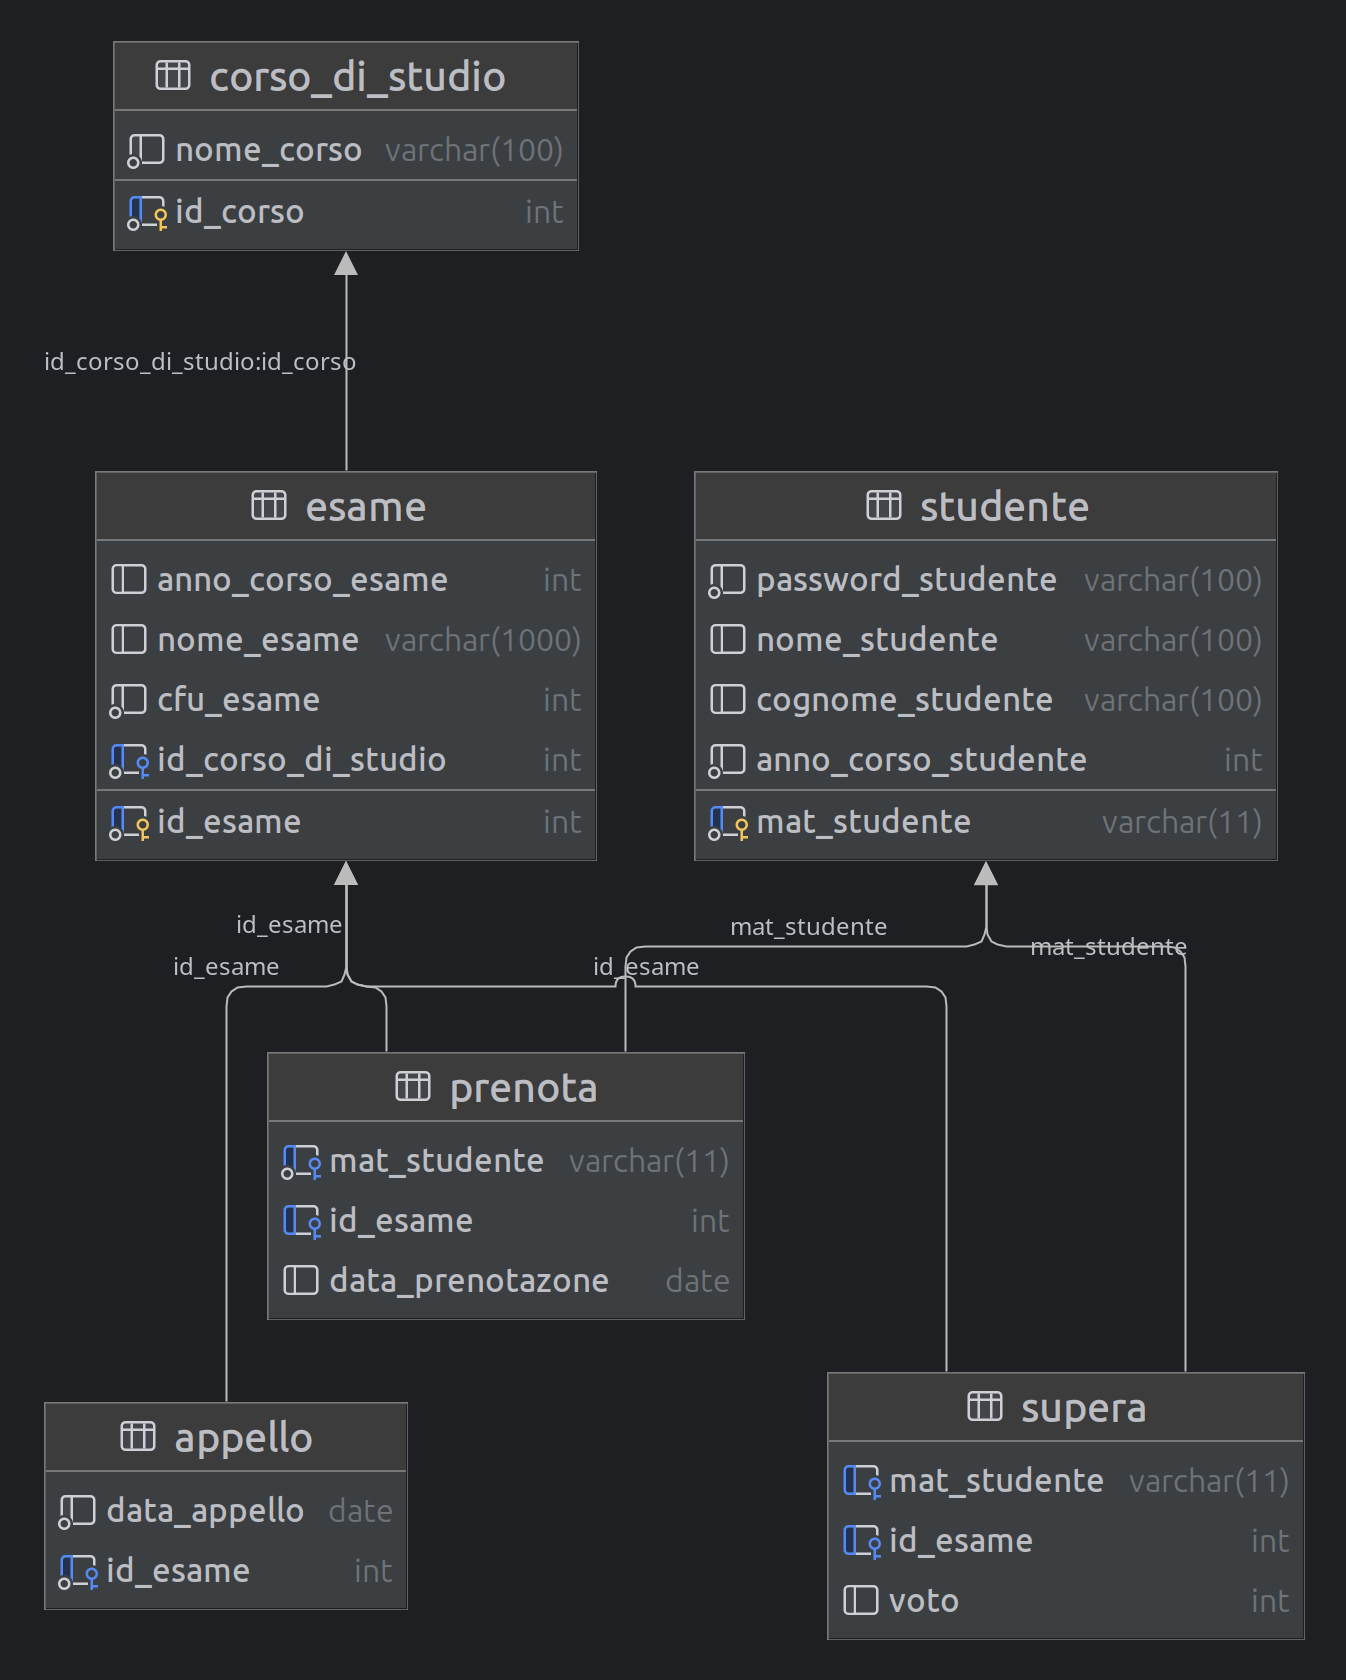
\includegraphics[width=0.7\textwidth]{universitaDB.png}
		\caption{Schema Database Univerisità}
		\label{fig:sdu}
		\end{center}
	\end{figure}
	
			
		

	
\end{itemize}

	
	
	\newpage
	\pagestyle{plain}
	
	
\end{document}
